\documentclass[preprint, floatfix, pra, showpacs, showkeys]{revtex4}
\usepackage{graphicx}
\usepackage{dcolumn}

\newcommand{\threej}[6]{\ensuremath{\left({#1\atop #4}{#2\atop #5}
{#3\atop #6}\right)}}
\newcommand{\sixj}[6]{\ensuremath{\left\{{#1\atop #4}{#2\atop #5}
{#3\atop #6}\right\}}}

\begin{document}

\title{The Flexible Atomic Code: IV. Autoionization and Dielectronic
Recombination}  
\author{Ming Feng Gu}
\affiliation{Center for Space Research, Massachusetts Institute of Technology,
Cambridge, MA 02139} 
\email[Email: ]{mfgu@space.mit.edu}

\begin{abstract} 
A computer program for calculating autoionization and radiationless electron
capture rates based on the relativistic distorted-wave and
isolated resonance approximations is presented. The method implements an
efficient 
interpolation procedure for the calculation of the autoionization radial
integrals. The 
autoionization rates of Ne-like selenium is calculated with the same
interacting configurations as in a previously published work for
comparison. Knowledge of autoionization and
radiationless electron capture rates enables one to treat various resonant
processes occurring in recombination, excitation, and ionization within
the distorted-wave framework. We illustrate its application in the calculation
of rate coefficients for dielectronic recombination of F-like iron to form
Ne-like iron. 
\end{abstract}

\pacs{32.80.Dz}
\keywords{Distorted-wave; Autoionization; Dielectronic recombination}
\maketitle

\section{Introduction}
In Ref.~\cite{gu02c}, we discussed
the calculation of non-resonant photoionization and radiative recombination
cross sections
using the Flexible Atomic Code (FAC). In many cases, the resonance
contributions to the recombination, excitation and ionization rates are
substantial or even dominate. Therefore, adequate interpretation of plasma
spectra from various laboratory and astrophysical sources require accurate
data for these resonant processes. 

The most accurate methods used today for treating resonances are ones based on
the close-coupling (CC) approximation, which yield unified results for both
background and resonant contributions. The efficient R-matrix implementation
of the CC approximation has been used extensively in the past to calculate
photoionization, recombination and electron impact excitation cross sections
\cite{hummer93, berrington95}. The main drawback of this approximation is
that it is very CPU-time consuming. Therefore, the number of coupled
channels are often limited in realistic calculations. Fortunately, in many
applications, especially for highly 
ionized ions, methods based on the distorted-wave (DW) approximation are
proven to be reasonably accurate even for resonant processes, e.g., as
indicated by the comparison between various DW calculations and experimental 
measurements of the dielectronic recombination (DR) rate coefficients for
O-like and F-like iron \cite{savin99}. In the DW methods, resonances are
usually treated as 
multi-step processes, one or more of these steps involve autoionization (AI)
or its inverse process, radiationless
electron capture. For example, the first step of DR is the radiationless
electron capture, followed by radiative decay, which competes with
autoionization. Therefore, the calculation of autoionization rates is the
major task in any DW treatments of resonant processes. Several DW programs
have been developed for this purpose in the past decades \cite{pindzola80,
kim87, oreg91}. The present method is most similar to that of
\textcite{oreg91}, which uses an efficient factorization-interpolation procedure
for the calculation of the autoionization radial integrals. 

In Section \ref{sec_theory}, we outline the theoretical background and discuss
the important numerical techniques used in the program. Section
\ref{sec_results} presents the calculated AI rates for Ne-like selenium, as
compared with the results of \textcite{oreg91}. In addition, 
the $\Delta n = 0$ DR rate coefficients of F-like iron are calculated and
compared with the experimental and theoretical results of \textcite{savin99}. 
Section \ref{sec_conclusions} gives a biref summary.

\section{Theory and Numerical Techniques}
\label{sec_theory}
In the first order perturbation theory, the AI rate can be written as (in
atomic units) 
\begin{equation}
A^a = 2\sum_\kappa \left|
<\psi_f,\kappa;J_TM_T|\sum_{i<j}\frac{1}{r_{ij}}|\psi_i>\right|^2,
\end{equation}
where $\psi_i$ is the autoionizing state, $\psi_f$ is the final state which has
one less electron than $\psi_i$, $\kappa$ is the relativistic angular quantum
number of the free electron, whose wavefunction is normalized as discussed in
Ref.~\cite{gu02b}. The total angular momentum of the coupled final state must
be equal to that of $\psi_i$, i.e.,  $J_T = J_i$ and $M_T = M_i$. After the
separation of the angular and radial integrals, we have
\begin{equation}
A^a = 2[J_i]^{-1}\sum_\kappa \left|\sum_{k,\alpha\gamma\delta}
<\psi_f,\kappa;J_T||Z^k(\alpha,\gamma)
\cdot Z^k(\kappa,\delta)||\psi_i>P^k(\kappa\delta;\alpha\gamma)\right|^2,
\end{equation}
where $\gamma$ and $\delta$ are the doubly excited bound orbitals in
$\psi_i$, $\alpha$ is the orbital which makes the internal transition in
$\psi_f$, and
$P^k$ is the radial integral as defined in the expression for the DW collision
strength of electron impact excitation, except that one of the free orbital
is replaced by a bound orbital \cite{gu02b}. For autoionization of
complex ions, the radial integrals $P^k$ with the same set of bound orbitals,
$\alpha$, $\gamma$, and $\delta$, 
often appear in many different transitions. However, the energies of the free
electrons in these integrals are different due to the conservation of
energy. It is 
computationally demanding to calculate such integrals for each transition
individually. Fortunately, the dependence of $P^k$ on the free electron energy
is rather weak, as noticed by \textcite{oreg91}. Therefore, it is possible to
calculate $P^k$ at a few energies, and the integrals at actual transition
energies are obtained by interpolation from these values. Usually, for a given
class of 
transitions, a three-point grid spanning the entire range of transition
energies is sufficient.

The inverse process of AI is radiationless electron capture, or sometimes,
called dielectronic capture (DC). The cross sections for DC are related to AI
rates through the detailed balance. DC is a resonant process which only occur
at certain energy. These resonances are extremely narrow, and in most
applications, it is more appropriate to characterize each resonance by its
resonance strength, which is the cross section integrated over energy. In
atomic units, the DC strength can be written as
\begin{equation}
S_{DC} = \frac{g_i}{2g_f}\frac{\pi^2}{E_{if}}A^a,
\end{equation}
where $g_i$ and $g_f$ are the statistical weights of the autoionizing state
formed by DC and the target state before DC, respectively, and $E_{if}$ is the
resonance energy. 

The autoionizing state formed by DC may either autoionize, or radiatively
decay. Radiative decay to the states below the ionization limit completes the
recombination process, DR. Sometimes, the final state of decay lies above the
ionization limit, and may further decay to yield DR or autoionize. Therefore,
the radiative branching ratio for DR can be expressed as
\begin{equation}
\label{eq_B}
B(i) = \frac{\sum_k A^r(i\to k) + \sum_a A^r(i\to a)B(a)}
{\sum_{k^\prime}A^a(i\to k^\prime) + \sum_k A^r(i\to k) + \sum_a A^r(i\to a)},
\end{equation}
where $A^r$ represents radiative decay rates, $k$ denotes levels below the
ionization limit, $a$ denotes levels which 
may further autoionize, and $k^\prime$ are the final levels of
autoionization. In most cases, the effect of radiative decay to autoionizing
levels is small, an approximate expression for the branching ratio may be used
by dropping the final term in both the numerator and denominator of
Eq.~(\ref{eq_B}), that is 
\begin{equation}
\label{eq_BApprox}B(i) = \frac{\sum_k A^r(i\to k)}
{\sum_{k^\prime}A^a(i\to k^\prime) + \sum_k A^r(i\to k)}.
\end{equation}
This approximation turns out to be fairly good even if the decay to
autoionizing levels is not completely negligible as demonstrated and explained
by \textcite{behar95, behar96}. The DR strength $S_{DR}$ is the product of DC
strength and the branching ratio.

In plasma modeling, the DR rate coefficients, $\alpha_{DR}$, for electrons in
the Maxwellian distribution is often needed, which can be expressed as
\begin{equation}
\label{eq_rate}
\alpha_{DR}(T) = \frac{h^3}{(2\pi m_e k_BT)^{3/2}}\sum_i\frac{g_i}{2g_f}
A^a(i\to f)B(i)\exp\left(-\frac{E_{if}}{k_BT}\right),
\end{equation}
where $T$ is the electron temperature, $m_e$ is the electron mass, $h$ is the
Planck constant, and $k_B$ is the Boltzmann constant. Since rate coefficients
are not fundamental atomic parameters, atomic units is not used in this
expression. 

The summation over the autoionizing levels $i$ in Eq.~(\ref{eq_rate})
extends to all possible states which may be formed by DC. Usually, the states
of each 
complex, designated as $nln^\prime l^\prime$, where the excited core electron
and the captured electron have the principal quantum numbers, $n$ and
$n^\prime$, are considered separately. 
The number of different $nl$ terms for the excited core
electron need to be considered is not large. Usually, the $\Delta n = 0$
resonances, where the transition of the core electron does not change its
principal quantum number, and $\Delta n = 1$ resonances, where the principal
quantum number of the core electron changes by one unit, make
dominant contributions to the 
total DR rate coefficients at temperatures of interest. The summation
over $n^\prime l^\prime$, however, can potentially involve large number of
terms. For high $n^\prime$, the contributions from large $l^\prime$ are
negligible. The maximum $l^\prime$ of 6--8 and $\sim 12$ are sufficient for
$\Delta n \ne 0$ and $\Delta n = 0$ resonances, respectively. The maximum
$n^\prime$ for $\Delta n \ne 0$ resonances is usually chosen to be $\sim 15$,
beyond which, the $n^{\prime -3}$ scaling law may be used for
extrapolation. For $\Delta n = 0$ resonances, the minimum $n^\prime$ which
opens some low energy channels can be large, and the $n^{\prime -3}$ scaling
law is only valid for very large $n^\prime$. Nevertheless, the partial DR rate
coefficients as a function of $n^\prime$ is quite smooth except for some
irregularities. Therefore, detailed 
calculations can be carried out on a suitable $n^\prime$ grid.
Interpolation may be used to complete the summation. However, one should pay
special attention to those $n^\prime$ where a specific channel starts to
open, because the rate coefficients is discontinuous at such $n^\prime$. In
addition, the rate coefficients of very low energy resonances are quite
sensitive to the exact value of the resonance energies. The theoretical
energies should be used with caution for resonances below a few tens of
eV. Sometimes, shifting the resonance energies for an entire series according
to the experimental transition energies of the core prove to be practical.

\section{Results}
\label{sec_results}
\subsection{Autoionization rates of Ne-like Selenium}
The autoionization rates for the selected configurations of Ne-like Se is
calculated. Only the doubly excited states of the Ne-like configurations, 
$2s^22p^43s^2$ and $2s^22p^43s3p$ are included for the purpose of comparison
with the results of \textcite{oreg91}. The Ne-like doubly excited
configurations are used to construct the optimal central potential. This is to
make the calculation 
more similar to that of \textcite{oreg91}, where the optimal potential is
determined by minimizing the energies of the doubly excited configurations.
The resulting AI rates are not very sensitive to the exact manner the potential
is determined. For example, using the ground configuration of the F-like ion
plus an $n = 3$ screening electron as the mean configuration results in
less than 10\% change for most transitions.

In Table \ref{tab_comparison}, we show AI rates to the two F-like
states, $2p_{1/2}2p^4_{3/2}$ and $2p^2_{1/2}2p^3_{3/2}$, calculated by the
present program. Two sets of results are shown, one is obtained by constructing
the mean configuration based on the doubly excited configurations, the other
has the mean configuration constructed by adding an $n = 3$ screening electron
to the ground configuration of the F-like ion. For comparison, the rates of
\textcite{oreg91} are presented as 
well. The difference between the two FAC results and those of \textcite{oreg91}
is mostly within a few percent, with a few exceptions of $\sim$ 10--30\%. 
 
\begingroup
\squeezetable
\begin{table}
\caption{\label{tab_comparison} The comparison of AI rates (in $10^{12}$
s$^{-1}$) for Ne-like selenium. The level labels are identical to those of
\textcite{oreg91}. 
The columns labeled by FAC$_1$ are the present results obtained with the mean
configuration constructed from the Ne-like doubly excited configurations, and
those labeled by FAC$_2$ have the mean configuration constructed by adding an
$n = 3$ screening electron to the ground configuration of the F-like ion. To
save the space, only the rates for autoionizing states having
$J = 0$, and $1$ are listed.}
\begin{ruledtabular}
\begin{tabular}{l*{7}{d}}
&&\multicolumn{3}{c}{$2p_{1/2}2p^4_{3/2}$}&
\multicolumn{3}{c}{$2p^2_{1/2}2p^3_{3/2}$}\\
\cline{3-5}\cline{6-8}
Level&\multicolumn{1}{c}{J}&\multicolumn{1}{c}{Ref.~\cite{oreg91}}&
\multicolumn{1}{c}{FAC$_1$}&\multicolumn{1}{c}{FAC$_2$}&
\multicolumn{1}{c}{Ref.~\cite{oreg91}}&
\multicolumn{1}{c}{FAC$_1$}&\multicolumn{1}{c}{FAC$_2$}\\
\hline
$(2p^2_{1/2}2p^2_{3/2})_03s^2$&0&0.85&0.80&0.78&13.3&13.1&13.2\\
$2p^4_{3/2}3s^2$&0&13.0&12.1&12.3&0.84&0.82&0.80\\
$[(2p^2_{1/2}2p^2_{3/2})_03s]_{1/2}3p_{1/2}$&0&0.003&0.002&0.002&0.21&0.25&0.23\\
$[(2p_{1/2}2p^3_{3/2})_13s]_{1/2}3p_{1/2}$&0&0.0&0.018&0.02&0.32&0.37&0.35\\
$(2p^4_{3/2}3s)_{1/2}3p_{1/2}$&0&168.0&168.0&164.0&0.03&0.038&0.037\\
$[(2p^2_{1/2}2p^2_{3/2})_23s]_{3/2}3p_{3/2}$&0&0.78&0.74&0.74&0.73&0.84&0.78\\
$[(2p_{1/2}2p^3_{3/2})_13s]_{3/2}3p_{3/2}$&0&5.96&6.84&6.89&0.21&0.22&0.22\\
$[(2p_{1/2}2p^3_{3/2})_23s]_{3/2}3p_{3/2}$&0&188.0&185.0&185.0&0.003&0.006&0.003\\
$(2p_{1/2}2p^3_{3/2})_13s^2$&1&7.11&6.98&7.06&6.96&6.52&6.58\\
$[(2p^2_{1/2}2p^2_{3/2})_03s]_{1/2}3p_{1/2}$&1&0.002&0.002&0.002&0.84&0.95&0.92\\
$[(2p^2_{1/2}2p^2_{3/2})_23s]_{3/2}3p_{1/2}$&1&0.13&0.12&0.11&0.50&0.57&0.54\\
$[(2p_{1/2}2p^3_{3/2})_23s]_{1/2}3p_{1/2}$&1&0.41&0.50&0.43&11.6&10.2&7.74\\
$[(2p_{1/2}2p^3_{3/2})_13s]_{3/2}3p_{1/2}$&1&0.78&0.75&0.56&10.5&9.75&6.08\\
$[(2p_{1/2}2p^3_{3/2})_23s]_{3/2}3p_{1/2}$&1&34.9&33.2&32.1&154.0&156.0&152.0\\
$(2p^4_{3/2}3s)_{1/2}3p_{1/2}$&1&152.0&153.0&150.0&3.21&3.54&3.33\\
$[(2p^2_{1/2}2p^2_{3/2})_03s]_{1/2}3p_{3/2}$&1&1.57&1.69&1.63&20.4&21.7&24.7\\
$[(2p^2_{1/2}2p^2_{3/2})_23s]_{3/2}3p_{3/2}$&1&0.34&0.34&0.34&1.25&0.94&0.86\\
$[(2p^2_{1/2}2p^2_{3/2})_23s]_{5/2}3p_{3/2}$&1&1.20&1.32&1.45&54.2&56.7&62.0\\
$[(2p_{1/2}2p^3_{3/2})_13s]_{1/2}3p_{3/2}$&1&1.71&1.54&1.62&6.90&6.65&5.96\\
$[(2p_{1/2}2p^3_{3/2})_13s]_{3/2}3p_{3/2}$&1&0.89&0.71&0.69&80.6&78.9&78.7\\
$[(2p_{1/2}2p^3_{3/2})_23s]_{3/2}3p_{3/2}$&1&0.15&0.12&0.11&8.57&7.29&8.56\\
$[(2p_{1/2}2p^3_{3/2})_23s]_{5/2}3p_{3/2}$&1&143.0&142.0&144.0&84.3&85.4&83.0\\
$(2p^4_{3/2}3s)_{1/2}3p_{3/2}$&1&64.3&66.0&65.1&3.02&3.08&2.97\\
\end{tabular}
\end{ruledtabular}
\end{table}
\endgroup

\subsection{$\Delta n = 0$ DR of F-like iron}
\begin{figure}
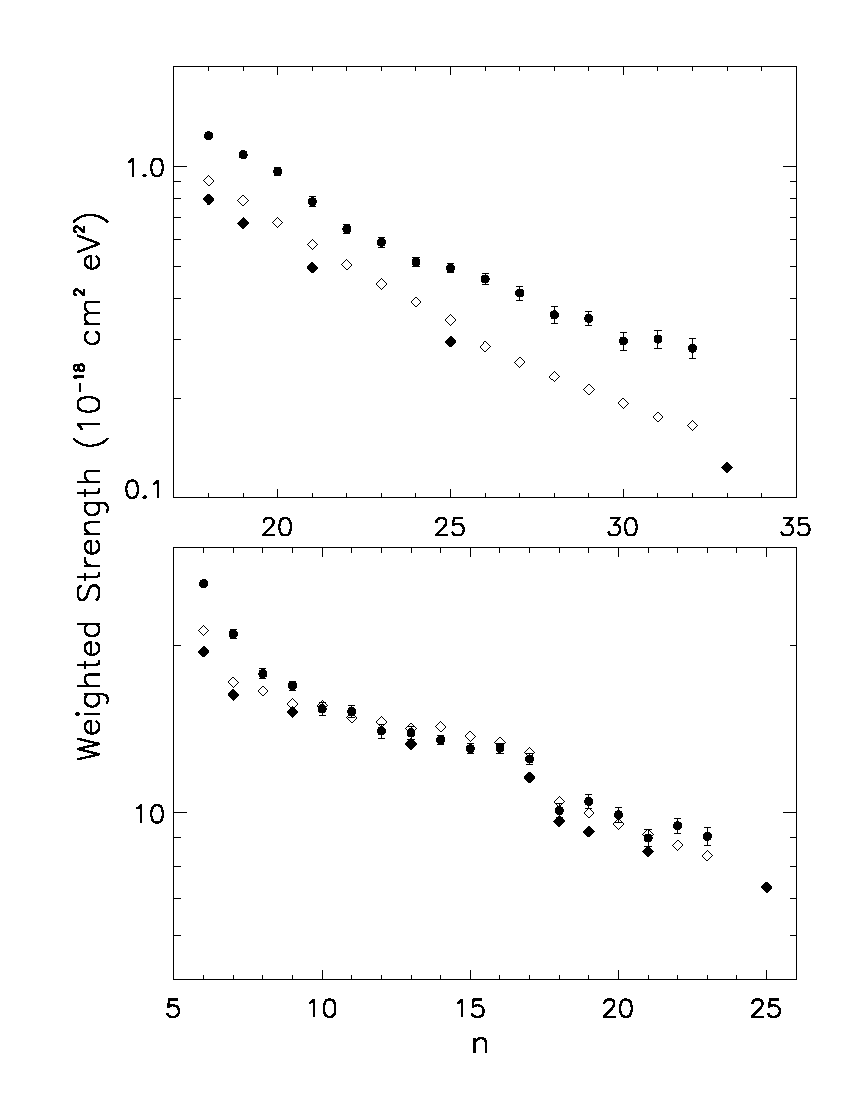
\includegraphics[width=5in]{str.eps}
\caption{\label{fig_str} Comparison of the energy weighted resonance
strengths of F-like iron. The top panel is for $P_{3/2}\to P_{1/2}$ channel,
the bottom 
panel is for $P_{3/2}\to S_{1/2}$ channel. The filled diamonds are the present
resuts, open diamonds and filled circles are the MCDF calculations and
experimental results of \textcite{savin99}. Note that the weighting factors of
the resonance strengths plotted in Figures 6 and 7 of \textcite{savin99} are that
of the highest energy resonances in each complex. The data plotted here
include a small corrections factor ($\sim$ 10\%) for the first three points in
both pannels.}
\end{figure}

\begin{figure}
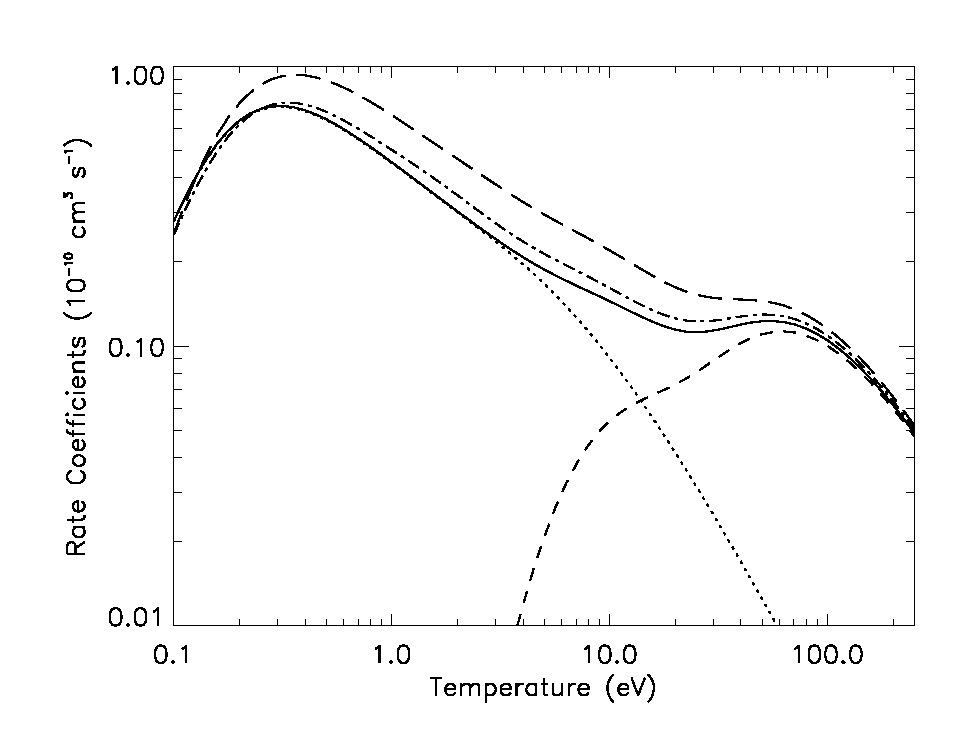
\includegraphics[width=5in]{rate.eps}
\caption{\label{fig_rate} Comparison of the $\Delta n = 0$ DR rate
coefficients of F-like iron. The dotted line is the present result for
$P_{3/2}\to P_{1/2}$ channel, the dashed line is the present result for
$P_{3/2}\to S_{1/2}$ channel, the solid line is the present total rate
coefficients, the dash-dotted and long-dashed lines are the MCDF calculations
and experimental results of \textcite{savin99}.}
\end{figure}

\textcite{savin99} have measured the $\Delta n = 0$ DR cross sections of O-like
and F-like iron 
using the heavy-ion Test Storage Ring, and compared the experimental results
with various theoretical calculations, all of them in the DW approximation. The
multi-configuration Dirac-Fork (MCDF) and Breit-Pauli (MCBP) calculations
presented in their paper are shown to agree with the measurement to within
20--30\%. Recently, \textcite{pradhan01} have calculated the $\Delta n = 0$ DR
of F-like iron using the CC approximation, and found to agree with the
experiment to within a similar percentage. 

In the present calculation, the target states of the F-like iron include the 
configuration mixing within the $n = 2$ complexes. There are only
two excitation channels for the $\Delta n = 0$ DR, corresponding to the core
transitions $2s^22p^5 P_{3/2}\to 2s^22p^5 P_{1/2}$ and $2s^22p^5 P_{3/2}\to
2s2p^6 S_{1/2}$, which have measured transition energies of 12.7182 and
132.0063 eV, respectively. The theoretical resonance energies are adjusted 
according to these experimental transition energies. The doubly excited states
of the Ne-like iron include the configuration mixing within the same
$nln^\prime l^\prime$ complex. 

The $P_{3/2}\to P_{1/2}$ channel starts to open at $n^\prime = 6$ for the
spectator electron, and the $P_{3/2}\to S_{1/2}$ channel starts to open at
$n^\prime = 18$. The orbital angular momentum $l^\prime$ of up to 12 are
included. Detailed calculations are carried out for $n^\prime =$6, 7, 9, 13,
17, 18, 19, 21, 25, 33, 49, and 60. DR rate coefficients for other values of
$n^\prime < 60$ are obtained by interpolation, and for $n^\prime > 60$ by
extrapolation using the $n^{\prime-3}$ scaling relation. 

In Figure \ref{fig_str}, we show the energy weighted resonance strengths as a
function of $n^\prime$. The strength for an entire $n^\prime$ complex is
calculated as 
\begin{equation}
S_n = \sum_i E_{if}S_{DC}B(i),
\end{equation}
which removes the trivial dependence on the resonance energies. The approximate
branching ratio given by Eq.~(\ref{eq_BApprox}) is used. 
Along with the present results, the MCDF calculations and the experimental
results of \textcite{savin99} are also shown. The present results seem to be
systematically lower than the MCDF calculations by $\sim$ 10--15\%, and 
both theoretical results are smaller than the measurements. 
Figure \ref{fig_rate} shows the comparison of total $\Delta n = 0$ DR rate
coefficients as a function of temperature. At temperatures above 100 eV, the
present calculations agree with the experimental results and the MCDF results
to within a few percent. At lower temperatures, the difference between the
present calculations and the MCDF results is less than 15\%, and the difference
between the present calculations and the measurements is $\sim$ 10--40\%.

\section{Conclusions}
\label{sec_conclusions}
A DW program is presented for calculating AI rates and DR rate
coefficients in the isolated resonance approximation. The interpolation of
autoionization radial integral in the continuum electron energy is implemented
to improve the efficiency. The calculated AI rates of Ne-like selenium are
in good agreement with previous theoretical calculations using comparable
approximations.  
The $\Delta n = 0$ DR strengths and rate coefficients of F-like iron are
compared with the recent MCDF calculations and storage ring measurements. 
The present results for DR rate coefficients of F-like iron agree with the
MCDF results and measurements to within a few percent at temperatures above
100 eV. At lower temperatures, the agreement is worse, $\sim$ 10--15\% with
the MCDF results and up to 40\% with the measurements.

\begin{acknowledgments}
The author would like to thank Ehud Behar for helpful discussions, and
Daniel Savin for providing the experimental and MCDF data in electronic
format. This work is supported by
NASA through Chandra Postdoctoral Fellowship Award Number PF01-10014 issued by
the Chandra X-ray Observatory Center, which is operated by Smithsonian
Astrophysical Observatory for and on behalf of NASA under contract NAS8-39073.
\end{acknowledgments}

\bibliographystyle{apsrev}
\bibliography{facref}

\end{document}

